We start by statically analyzing a random sample of cloud applications to learn various properties related
to branching, looping and usage of cloud SDK interfaces in the applications written for PaaS environments. 
We scour the GitHub source code repository for open source Google App Engine applications written in Java,
and randomly select a population of 35 applications. These applications are subjected to a thorough analysis
using the Soot framework to study their code patterns. Our analysis detected 1458 different methods in all the
applications. In this section we present a detailed overview of the observations made in this study. We note that
our design and implementation of Cerebro, and the associated experiments have been influenced by 
these observations in several ways.

\begin{figure}
\centering
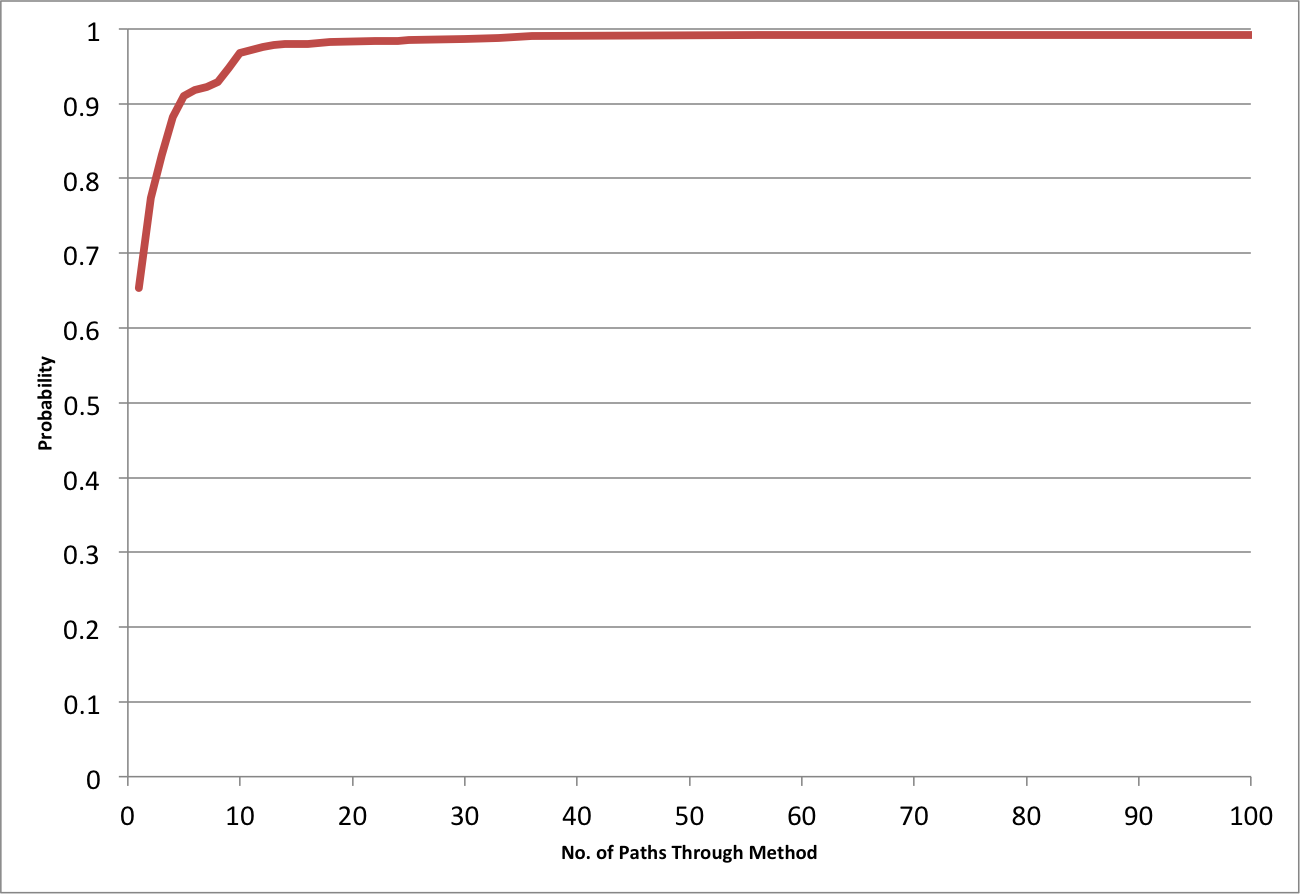
\includegraphics[scale=0.35]{path_count_cdf}
\caption{CDF of path counts through methods in web applications.}
\label{fig:path_count_cdf}
\end{figure}

FIgure~\ref{fig:path_count_cdf} shows the number of paths through methods, and the probability of encountering
a method with a given number of paths (in other words the branching behavior of methods). According to this CDF, 
around 97\% of the methods considered in the analysis have 10 or less paths going through them. About 99\% of 
the methods have 36 or less paths going through them. However, this CDF does have a very long tail, going all the way
up to 34992 (not shown in the figure -- the x-axis of the CDF has been truncated at 100 paths). Still, it is interesting to note that more
than half the methods considered in the analysis, 65\% to be precise, have no more than exactly 1 path (i.e. no branches).
This implies that roughly 65\% of the time, Cerebro has to only generate a single sequence of predictions. In cases
where there are multiple branches, Cerebro's unique path detection mechanism can help significantly 
reduce the number of prediction traces that need to be generated.

Next we look at the looping behavior of the 35 web applications used in the study. As it turns out 1286 of the methods (88\%)
considered in the study
do not have any loops. Only 172 methods (12\%) consist of loops. Clearly the PaaS SDK and the associated coding restrictions
are making loops a somewhat rare feature in the cloud applications. Around 29\% of all the loops found in 
the analyzed code do not contain any cloud SDK invocations. 
A large majority of the loops (61\%), however, are
used to stream a dataset from the datastore cloud SDK interface of Google App Engine (i.e iterating on the result set 
returned by a datastore query). We refer to this particular type of loops as iterative datastore reads. 
We use these vital pieces of information when designing the loop handling capability of
Cerebro.

\begin{table}[htdp]
\caption{Number of times different cloud SDK interfaces are called in web applications.}
\begin{center}
\begin{tabular}{|c|c|}
\hline
Cloud SDK Interface & No. of Invocations \\ \hline
blobstore & 7 \\ \hline
channel & 1 \\ \hline
datastore & 735 \\ \hline
files & 4 \\ \hline
images & 3 \\ \hline
memcache & 12 \\ \hline
search & 6 \\ \hline
taskqueue & 24 \\ \hline
tools & 2 \\ \hline
urlfetch & 8 \\ \hline
users & 44 \\ \hline
xmpp & 3 \\ \hline
\end{tabular}
\end{center}
\label{tab:sdk_call_counts}
\end{table}

Table~\ref{tab:sdk_call_counts} lists the number of times each cloud SDK interface has been called in the sample of
35 web applications. Clearly datastore is the most commonly used interface as far as Google App Engine applications are 
concerned. This is because data storage and access is a fundamental capability required by most web applications. 
Some of the other widely used interfaces include users, taskqueue and memcache. 

\begin{figure}
\centering
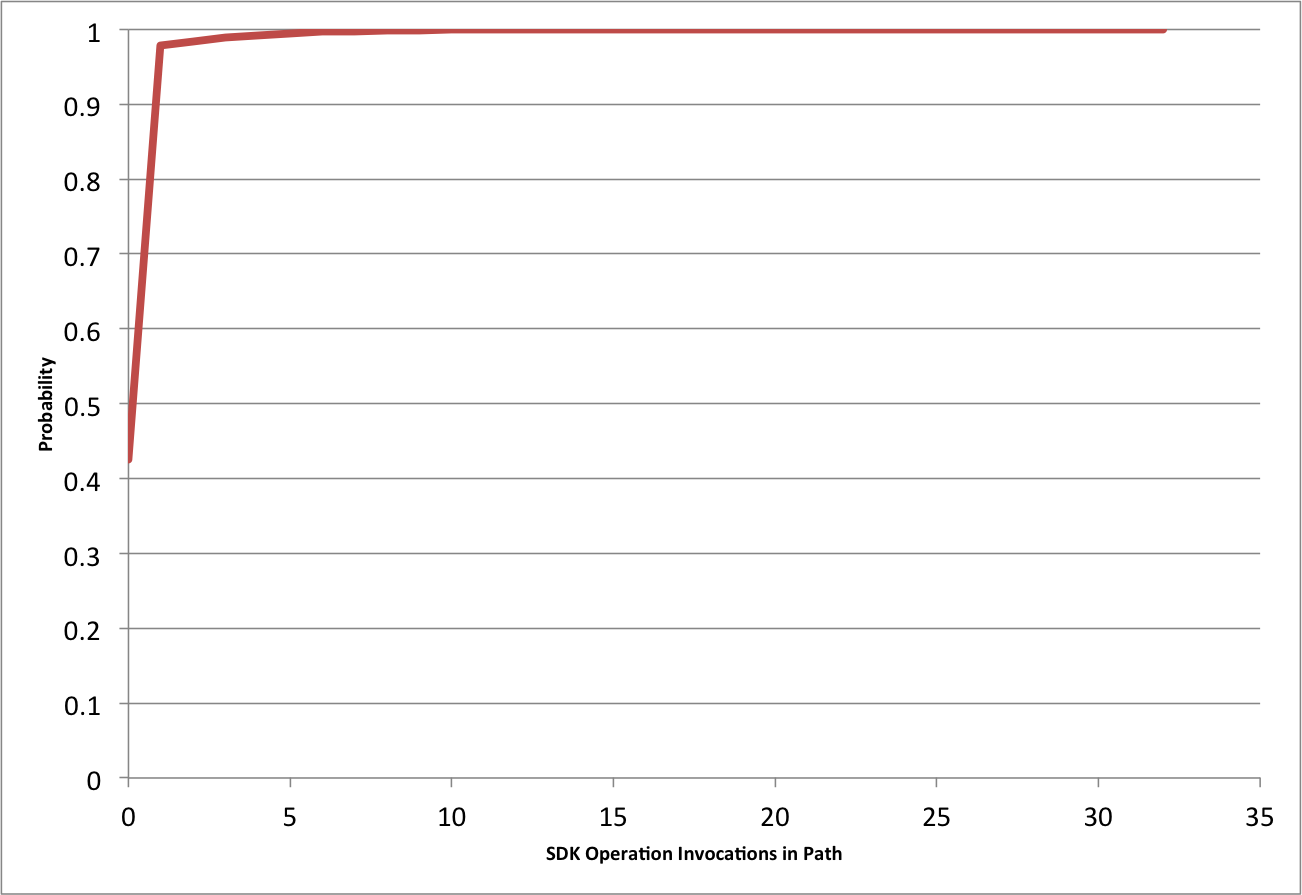
\includegraphics[scale=0.35]{sdk_call_count_cdf}
\caption{CDF of cloud SDK call counts in web applications.}
\label{fig:sdk_call_count_cdf}
\end{figure}

Finally we explore the number of cloud SDK calls made in different paths of execution in the web applications. For this study
we consider all the paths of execution through the methods. This amounted to 64780 total paths. Figure~\ref{fig:sdk_call_count_cdf}
shows the number of cloud SDK calls in the paths, and the probability of finding a path with a given number of cloud SDK calls.
According to that around 98\% of the paths have 1 or less cloud SDK call. The probability of finding an execution path with more than
5 cloud SDK calls is smaller than 0.01. This implies in most cases Cerebro will make response time predictions without having to 
aggregate multiple time series together.